\subsection{ArduinoDesign.}    

The prototype is designed to prove the concept of the requirements to direct the power to and away from the media, control a tag reader, communicate with the server and it need to be an embedded system. \newline

\begin{figure}[h]
	\centering
		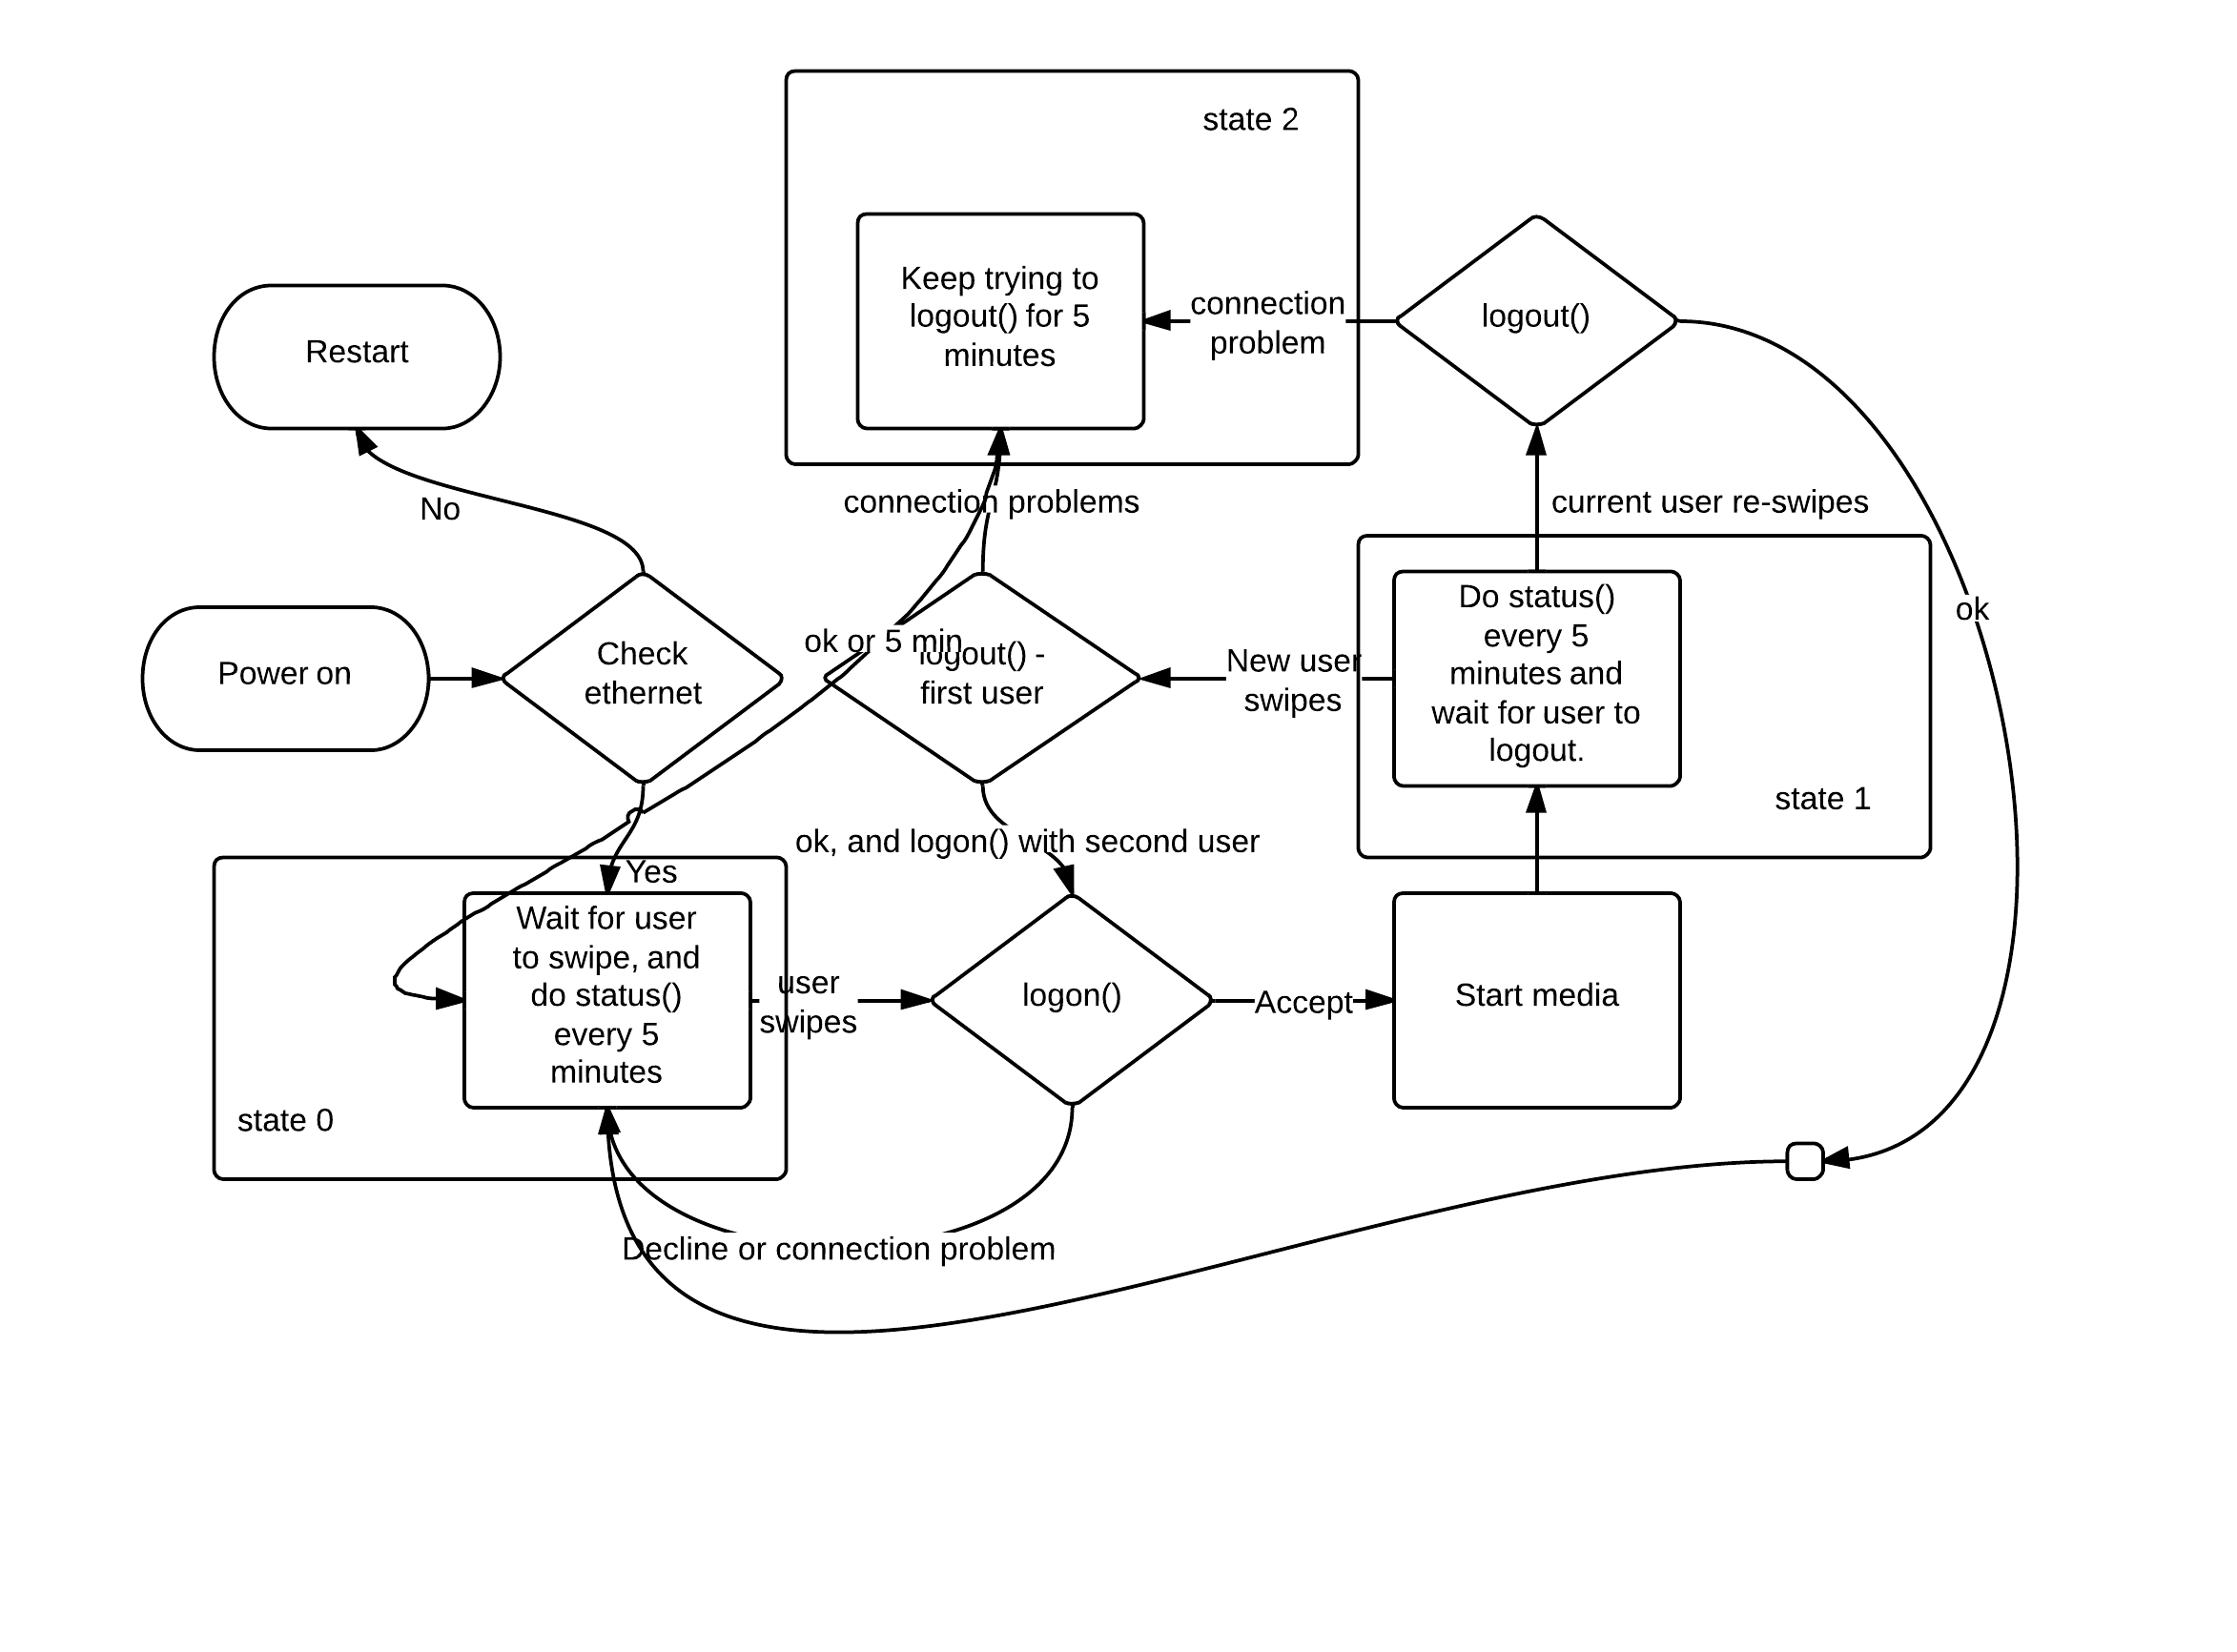
\includegraphics[width=1.50\textwidth, angle=90]{images/arduinoFlowchart.png}
	\caption{Simple Flowchart of Arduino}
	\label{fig:arduinoFlowchart}
\end{figure}

As described in section \ref{chap:controller} it is only parts of the visioned system that is implemented in  the Arduino. 
To illustrate and describe this functionality a simplified flowchart and a short description of it has been made, see figure \ref{fig:arduinoFlowchart},. The boxes of state in the Arduino flowchart will be described in section \ref{ProgrammingBasicsforArduino}.
The functions in focus for implementation on the Arduino is: 

\begin{itemize}
	\item Read and accept/decline tags in communication with a server through an online connection.
	\item Monitor and handle the server connection.
	\item Regulate the power according to the scenario.
	\item Manage the time usage and user restrictions. 
	%\item Communicate system status to user through LED light indication. 
\end{itemize}

Starting up the Arduino is setting up the Ethernet connection and the pins to lights and RFID shields. If the connection can not be established  the Arduino will need to restart. This start up phase is not similar to the expected setting up phase described in \ref{subsec:senarioD} and shall therefor not be evaluated as the end system solution.

For the most part the system is looking for tags, checking user restriction and every 5 minutes receiving updates from the database server through a \verb|getStatus()| call. \\
The status call keeps the Arduino updated on changes in rules or time the user may spent at the device.      
For most scenarios of disconnection from the server the Arduino will return to this state, after attempting to handle the connection error.
Disconnection at log out will make the Arduino keep trying the log out procedure until accomplished, or if 5 minutes passes before a success it will return to the normal \verb|getStatus()| procedure. Because the server at that point will have logged the user off.
Almost the same happens, in the scenario of when a disconnection happens at status call with a user logged on. Then the Arduino have 3 minutes to reconnect before logging off the user, not on the server but by itself. 

The system is capable of switching users on the Arduino. But will result in the second user shutting down the media device the current user is using even though the new user do not have permission to use the media. The optimal solution is described in the user scenario, see \ref{Logonlogoffmedia}, where the API checks the permission of the new user before the Arduino takes action.       
